\documentclass[12pt]{article}

\usepackage{fullpage}
\usepackage{graphicx, rotating, booktabs} 
\usepackage{times}
\usepackage{fbb} 
\usepackage{natbib} 
\usepackage{indentfirst} 
\usepackage{setspace}
\usepackage{grffile} 
\usepackage{hyperref}
\usepackage{adjustbox}
\usepackage{multirow} 
\usepackage{amsmath}
\usepackage[labelfont={bf},textfont=it,labelsep=period]{caption}
\setcitestyle{aysep{}}
\usepackage{sectsty}
% for the big table
\usepackage{afterpage}
\usepackage{array}
\usepackage{lscape}
\usepackage{longtable}
\usepackage{float}
\sectionfont{\Large}
\subsectionfont{\noindent\large\textit}
\subsubsectionfont{\normalsize}


\singlespace
\title{\textbf{Appendix: Using Bayesian Hierarchical Models to Estimate Heterogeneous Effects}}
%\author{Joshua Alley} 
\date{}

\bibliographystyle{apsr}

\begin{document}

\maketitle 

\singlespace 

\tableofcontents

\bigskip





\section{Bush and Prather Reanalysis}


In the following, I demonstrate how the model works by reanalyzing a study by \citet{BushPrather2020} (BP hereafter). 
This study examines how foreign meddling in elections impacts support for economic engagement with the meddler. 
One of their experiments examines how Russian or German engagement in the 2016 US election impacts mass support for trade and investment with those countries.
I use a heterogeneous effects model to check their results and further explore their findings. 


% describe design
BP employ a 2x2x2 factorial experiment.
This design randomizes whether a foreign country is interfering in the 2016 election, the country and their attitude towards Trump and whether the potential economic ties entail greater trade or investment in the United States.
In one treatment, Russia expresses support for Trump and in the other, Germany expresses opposition to Trump. 


BP hypothesize that individuals will prefer economic engagement with states that support their candidate. 
They thus examine how the impact of side-taking varies with the direction of the endorsement, individual political preferences, and the economic issue. 
To do this, they use four tables and figures, and rely on eight t-tests of differences in means between groups of roughly 25 respondents. 


The heterogeneous effects model encapsulates the argument and all tests by estimating the impact of side-taking on economic engagement as a function of which country is involved, a dummy indicator of intention to vote for Clinton, and their interaction. 
The interaction captures the hypothesis that Clinton voters will support engagement with Germany because Germany opposed Trump, and should be positive. 
I also add an indicator of whether the experiment deals with trade or investment. 
Last the heterogeneous effects equation also includes indicators of female gender, active employment, college education, political knowledge, and political interest. 



The outcome variable is a scale from one to four that measures support for greater economic engagement with the potential partner. 
To approximate BP's analyses, I use a normal outcome likelihood. 
Because this experimental randomization produced a roughly balanced sample, I do not include any control variables in the outcome equation. 


\begin{figure}[htpb]
	\centering
		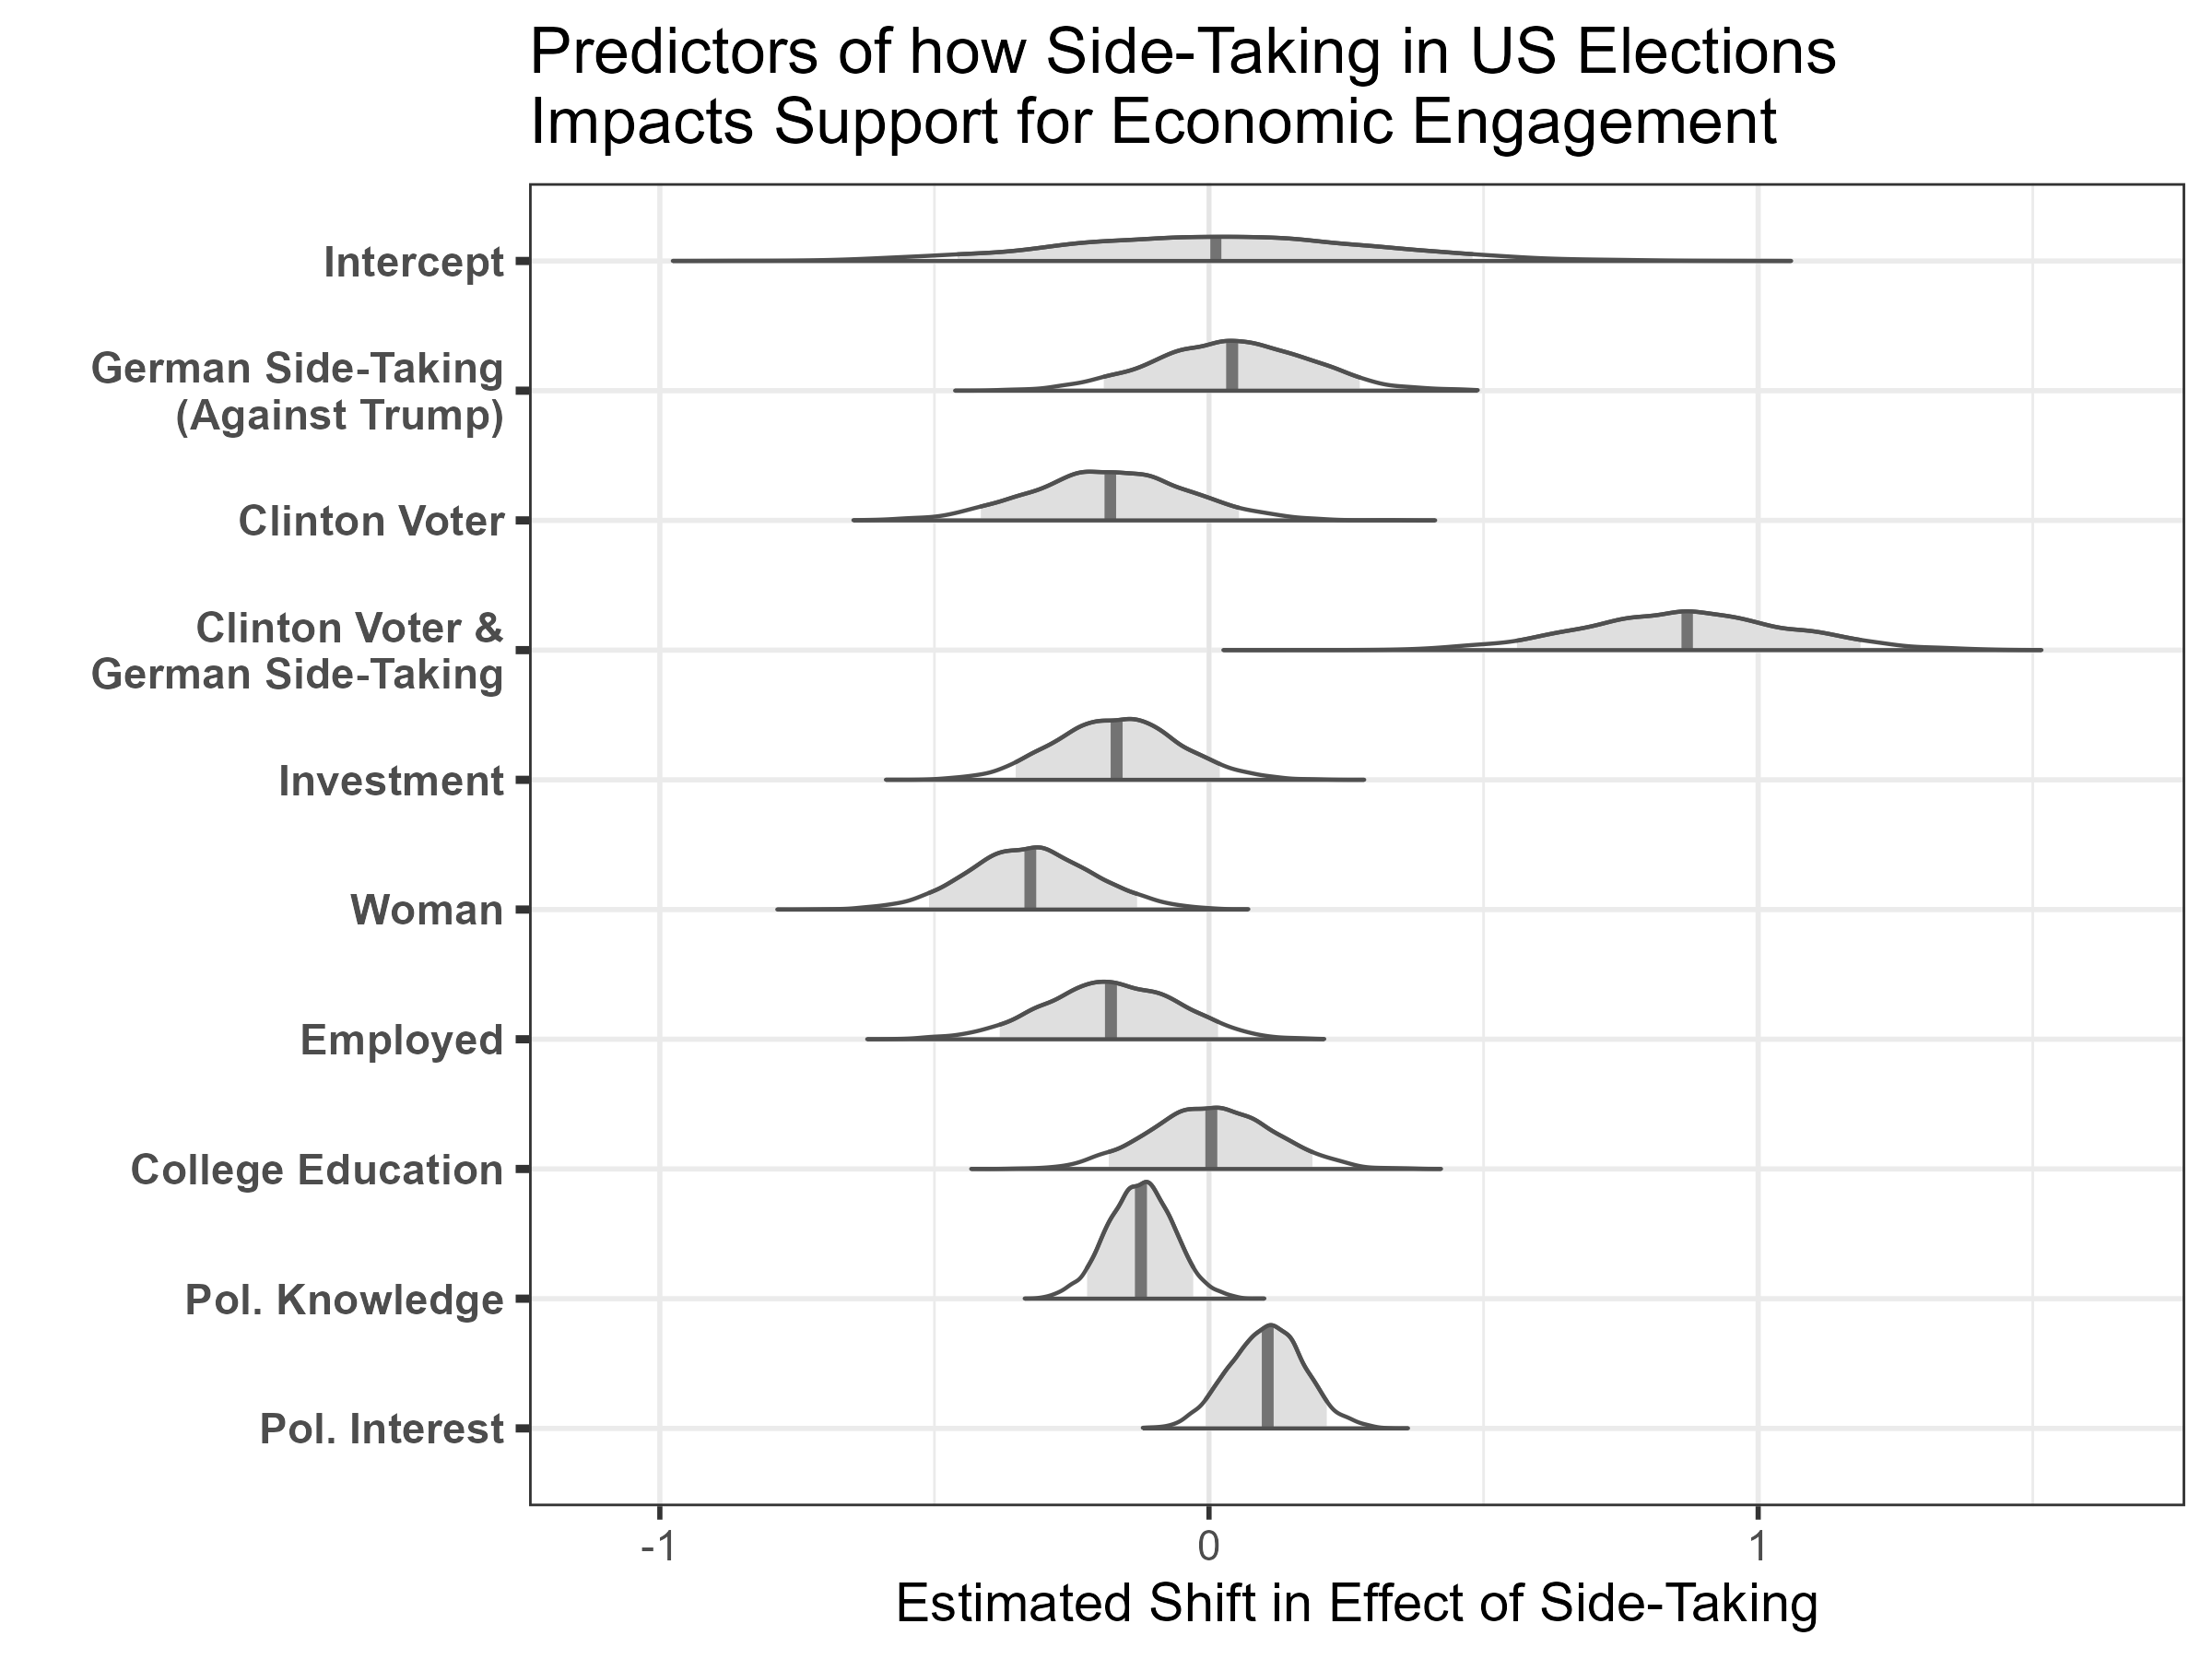
\includegraphics[width=0.95\textwidth]{../figures/bp-lambda.png}
	\caption{}
	\label{fig:bp-lambda}
\end{figure}


\autoref{fig:bp-lambda} summarizes the estimates from the heterogeneous effects equation. 
As BP predicted and find, side-taking increases support for economic engagement with voters whose candidate the intervention supports. 
Relative to the impact of Russian side-taking on Trump voters, German side-taking increases the impact of side taking by almost 1, which is a large difference on an outcome that ranges from 1 to 4. 
German side-taking does not impact Trump voter support for economic engagement, and Clinton voters are marginally but not clearly less supportive of engagement with Russia after Russian side-taking.
These estimates are consistent with BP's results. 


\begin{figure}[htpb]
	\centering
		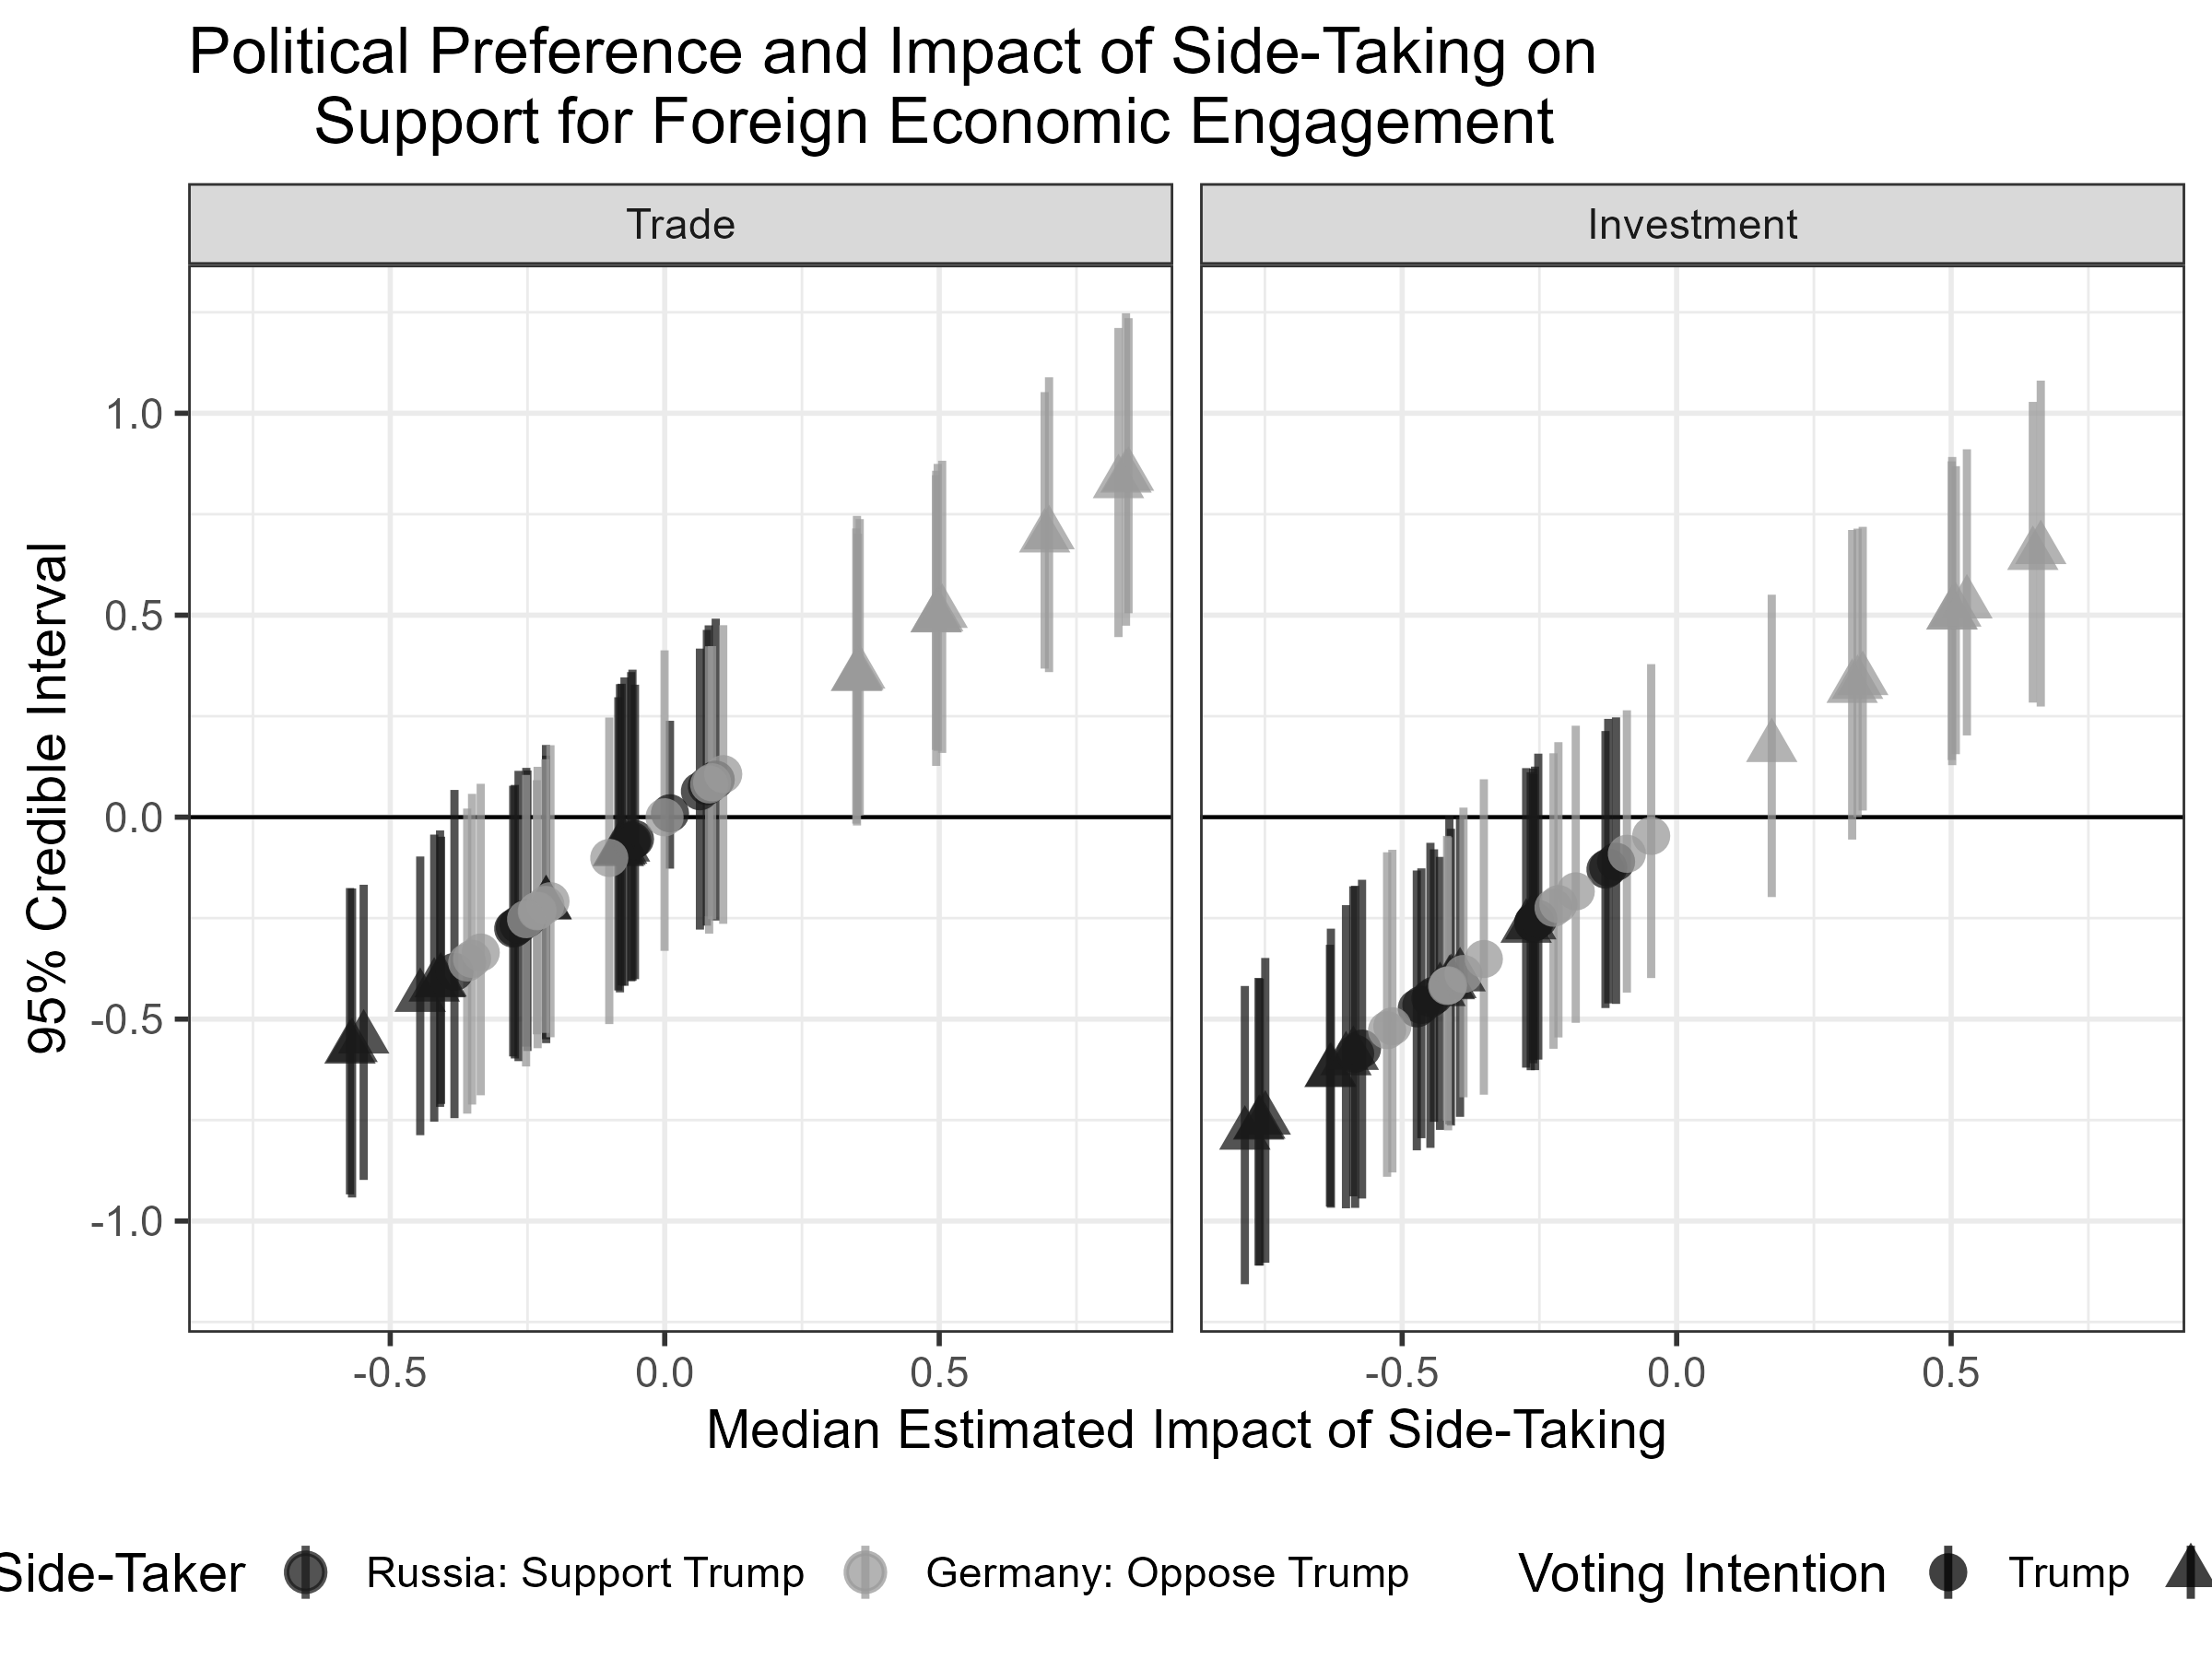
\includegraphics[width=0.95\textwidth]{../figures/bp-theta-est.png}
	\caption{Heterogeneous effects of foreign side-taking in US elections on support for economic engagement with the interfering country. Each estimate reflects a treated group with a unique combination of other treatments and demographic characteristics.}
	\label{fig:bp-theta-est}
\end{figure}


The model also provides some new information about how side-taking impacts support for economic engagement. 
Electoral side-taking is more likely to reduce support for foreign investment in the United States, all else equal. 
Moreover, women largely respond more negatively to side-taking. 
Finally, increasing political knowledge decreases the the impact of side-taking, while interest in politics increases it. 


\autoref{fig:bp-theta-est} substantiates these inferences and presents the group-specific treatment effects. 
In general, Clinton voters were more responsive to side-taking. 
Most Clinton voters were less likely to support trade and investment with Russia after exposure to Russian support for Trump, and more likely to back economic cooperation with Germany in response to German opposition to Trump. 
Additional variation in this relationship comes from gender and political engagement.
Some Trump voters reduce their support for investment regardless of who the intervention backs and are less likely to change their trade attitudes in response to side-taking as well. 


% power point
The credible intervals on these estimates suggest that researchers should not rely on this technique to generate powerful tests between groups, unless predictors of heterogeneous effects create substantial differences. 
For instance, most Trump voters hold very similar views of economic engagement, and there are only a few that are clearly different. 
Among Clinton voters, however, the response to German side-taking and corresponding distaste for Russian side-taking creates huge differences between different treated groups. 





\newpage
\singlespace
 
\bibliography{../../MasterBibliography} 


\end{document}